\chapter{Math}

\section{Filter}



\section{Trigonometrys}

\begin{center}
    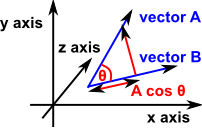
\includegraphics[width=0.4\textwidth]{images/dotProduct.png}
    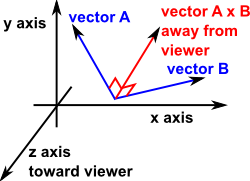
\includegraphics[width=0.4\textwidth]{images/crossProduct.png}
\end{center}


\section{Solid Rotations}

部分内容参考Euclidenan Space网站\cite{Euclideanspace}。

\subsection{Axis Angle}

任意3D旋转都可以表示,给一个solid对象,朝向orientation1,再给另一个朝向orientation2,可以总是
找到一轴axis和一角度angle从orientation1旋转到orientation2.

这个方法是好理解,但是把多个序列的旋转的结果就不好表示了,就需要使用matrix或quaternion啦

\subsection{Euler Angles}
把任意3D旋转分解decompose为三个不同的角度,直觉上会认为这种方式很方便,可是计算上会出现问题,如死锁


当合并旋转时,只有明确旋转顺序order才能确定Euler Angle的姿态。
\begin{description}
    \item [Tait-Bryan angles] \textsf{正序xyz, yzx, zxy; 反序zyx, xzy, yxz。在SLAM(simultaneous localization and mapping)同步定位与建图中应用}
    \item [Proper Euler angles] \textsf{xyx, xzx, yxy, yzy, zxz, zyz,}
\end{description}

旋转的参考,分内旋与外旋。假设世界坐标系XYZ与物体坐标系xyz重合,定义旋转顺序zyx,
旋转角度分别为$\theta, \phi, \psi$。先绕z轴旋转$\theta$后,物体的xy轴发生变化了,z轴不变。
现在旋转第二个旋转角y轴的$\phi$,此时需要内旋与外旋的概念来区分:内旋就是按照物体的坐标系的y轴来旋转,
外旋就是按照世界坐标系的Y轴来旋转。
旋转完成后,第三个旋转角也是如此。

这样一来,Euler Angle的旋转就的必要条件就是有:旋转角度,旋转顺序,旋转方式(内旋还是外旋)。

\begin{center}
    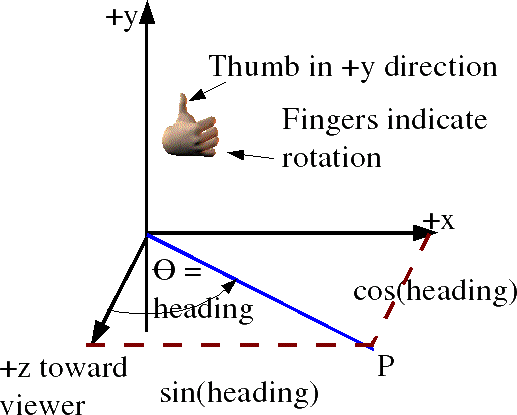
\includegraphics[width=0.3\textwidth]{images/heading.png}
    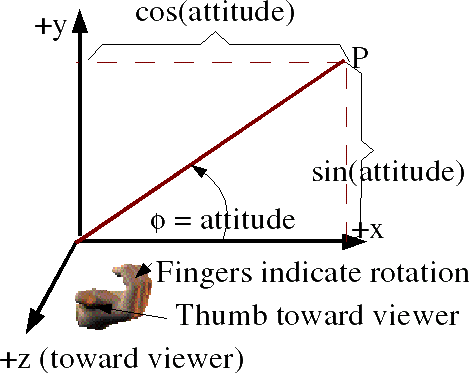
\includegraphics[width=0.3\textwidth]{images/attitude.png}
    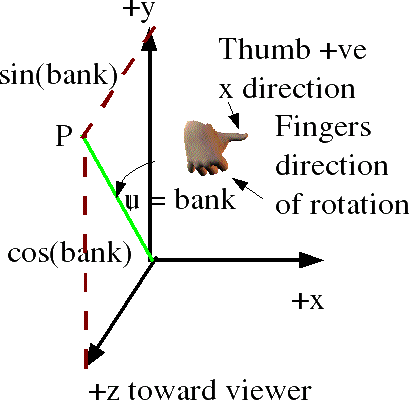
\includegraphics[width=0.3\textwidth]{images/bank.png}
\end{center}

\begin{tabular}{|c|c|c|c|c|c|}
    \hline
  & airplane & telescope & symbol & \hbox{angular velocity} & axis \\ \hline
 \hbox{applied first} & heading & azimuth & \hbox{$\theta$(theta)} & \hbox{yaw偏航} & X \\ \hline
 \hbox{applied second} & attitude & elevation & \hbox{$\phi$(phi)} & \hbox{pitch俯仰} & Z \\ \hline
 \hbox{applied last} & bank & tilt & \hbox{$\psi$(psi)} & \hbox{roll横滚} \\ \hline
\end{tabular}
 
 欧拉角的是为了方便主观去理解,与Axis Angle类型,以理解为主要入手处。

 
 \section{Linear-Transform}

线性变换主要包括缩放、旋转、反射等,不包含平移。线性变换的数学描述为:

\begin{math}
\begin{aligned}
f(\alpha v)=\alpha v, \\
f(u+v)=f(u)+f(v)
\end{aligned}
\end{math}

反射,就是把一个物体变换成它的镜像的映射,在二维空间中,用一条直线作为“镜子”;在三维空间中,使用平面作为“镜子”。


\section{ Matrix }

矩阵Matrix就是线性变换

\subsection{eigenvector}
特征向量
对于一个给定的线性变换(矩阵M,是向量空间E到自身的一个线性变换,可以旋转、反射、拉伸、压缩或变换的组合),它的特征向量V经过这个线性变换之后,得到新的向量U,VU向量共线,但长度可能不一致。
VU的长度缩放的比例称为特征值eigenvalue。

\subsection{minor}
余子式
在n阶行列式D中划去任意选定的k行、k列后,余下的元素按照原来的顺序组成的n-k阶行列式M,M称为
行列式D的k阶子式A的余子式Minor。如果k阶子式A在行列式D中的行和列的标号分别为
$i_{1},i_{2},...,i_{k}$和$j_{1},j_{2},...,j_{k}$。则在A的余子式M前面加一个符号:
\begin{math}
    \begin{aligned}
        {-1}^{(i_{1}+i_{2}+...+i_{k}) + (j_{1}+j_{2}+...+j_{k})}
    \end{aligned}
\end{math}
得到的n-k阶行列式,称为行列式D的k阶子式A的代数余子式Cofactor。

\subsection{determinant}
行列式
行列式其实是一个函数,一个将方阵转换成一个标量的函数。行列式可以看做是有向面积的概念在一般的欧几里得空间中的推广。
行列式表示的是线性变换前后的面积(二维)、(三维为体积)等变化的系数。

n阶行列式det(D)等于其任意行(列)的元素与对应的代数余子式的乘积之和。通过D的i行row来计算

\begin{math}
    \begin{aligned}
   \det(D)=d_{i1}A_{i1}+...+d_{in}A_{in}=\sum_{j=1}^{n}{a_{ij}(-1)^{(i+j)}A_{ij}}
    \end{aligned}
\end{math}

又称为拉普拉斯展开式Laplace expansion,或代数余子式展开式Cofactor expansion
矩阵和行列式是两个完全不一样的概念,行列式的行和列必须相等。

\subsection{adjoint matrix}
伴随矩阵
行列式D的每个元素的代数余子式$A_{ij}$所构成的矩阵,称为矩阵D的伴随矩阵。

\begin{math}
    \begin{aligned}
A^{*}= \begin{pmatrix} A_{11}&A_{21}&A_{...}&A_{n1} \\
A_{12}&A_{22}&A_{...}&A_{n2} \\
A_{...}&A_{...}&A_{...}&A_{...} \\
A_{1n}&A_{2n}&A_{...}&A_{nn} \end{pmatrix} = (A_{ij})^T
\end{aligned}
\end{math}

伴随矩阵就是线性变换的逆操作,再进行一个缩放的结果,缩放的大小与矩阵的行列式的值有关。
伴随矩阵定理:
A是n阶方阵,$A^*$是A的伴随矩阵,则有$AA^*=A^*A=AE$。

\subsection{inverse matrix}
逆矩阵
n阶方阵A,存在n阶方阵B,满足$AB=BA=E$,称方阵A可逆,称方阵B是A的逆矩阵,记为$B=A^{-1}$

由伴随矩阵定理与逆矩阵可得

\begin{math}
    \begin{aligned}
\begin{cases} A^*A=E\\ AA*=|A|E \end{cases} \Rightarrow A^{-1}=\frac{A^*}{|A|}
\end{aligned}
\end{math}


\subsection{正交矩阵}
两个向量的内积为零,就说这两个向量是正交的,在三维空间中,正交的两个向量相互垂直。如果相互正交
向量的长度均为1,又叫做标准正交基。
在矩阵论中,\textbf{实数}正交矩阵是方块矩阵Q,它的转置矩阵是它的逆矩阵,$Q^TQ=QQ^T=I$。
注意实数二字,正交矩阵中的元素都是实数,包含复数并且同样满足正交性质的矩阵是酉矩阵,也就是推广
到复数域之后的“正交矩阵”。

\subsection{相似矩阵}
两个n阶方阵矩阵A与B为相似矩阵当且仅当存在一个n阶方阵的可逆矩阵P,使得$P^{-1}AP=B$或$AP=PB$,
P被称为矩阵A与B之间的相似变换矩阵。
白话就是,矩阵是线性空间中的线性变换的一个描述,在一个线性空间中,只要我们选定一组基,那么对于
任何一个线性变换,都能够用一个确定的矩阵来加以描述。同样的,对于一个线性变换,只要逆选定一组基,
那么就可以找到一个矩阵来描述这个线性变换。换一组基,就得到一个不同的矩阵。所有这些矩阵都是这
同一个线性变换的描述,但又都不是线性变换本身。所有这些同一个线性变换的描述的矩阵互为\textbf{相似矩阵}。

\subsection{过渡矩阵}
transition matrix过渡矩阵这个词在数学语境中有很多地方用得,在线性代数中,它用来表示坐标矩阵的变换。
\newline
设V为n维向量空间,有两个基$S=\{v_1,...,v_n\}$和$T=\{w_1,...,w_n\}$,
过渡矩阵$P_{S \leftarrow T}$从T到S的nxn矩阵,它的列项在基S中的形式为:

\begin{math}
    P_{S \rightarrow T} = [[w_1]_S [w_2]_S ... [w_n]_S]
\end{math}

举例说明:设$S=\{ e_1,e_2,e_3\}$为标准基,$T=\{ w_1=\begin{bmatrix} 1\\ 1\\ 0 \end{bmatrix}\quad, w_2=\begin{bmatrix}0\\1\\2\end{bmatrix}\quad 
, w_3=\begin{bmatrix} 1\\1\\1 \end{bmatrix}\quad \}$。

则有\newline
$P_{S \leftarrow T}=\begin{bmatrix} 1&0&1\\1&1&1\\0&2&1\end{bmatrix}$。

根据这个关系,可以表示$w_3=2e_2+e_3$。

具体数值的例子:设$S=\{ v_1=\begin{bmatrix}1\\2\\3\end{bmatrix}\quad, v_2=\begin{bmatrix}-2\\1\\0\end{bmatrix}\quad 
, v_3=\begin{bmatrix} 1\\0\\1 \end{bmatrix}\quad \}$, $T=\{ w_1=\begin{bmatrix} 1\\1\\0\end{bmatrix}\quad, w_2=\begin{bmatrix}0\\1\\2\end{bmatrix}\quad 
, w_3=\begin{bmatrix} 1\\1\\1 \end{bmatrix}\quad \}$。

求得在基S中的$w_1$的坐标值$x_1,x_2,x_3$。
\newline
由线性关系可得

\begin{math}
    x_1v_1+x_2v_2+x_3v_3=w_1
\end{math}

它的增广矩阵为
\begin{math}
    [ { \begin{array}{c:c:c:c} 
        \begin{matrix} v_1&v_2&v_3 \end{matrix} &
        \begin{matrix} w_1 \end{matrix} &
        \begin{matrix} w_2 \end{matrix} &
        \begin{matrix} w_3 \end{matrix} 
    \end{array}} ] = \Bigg [ {\begin{array}{c:c:c:c} 
        \begin{matrix} 1&-2&1\\2&1&0\\3&0&1 \end{matrix} &
        \begin{matrix} 1\\1\\0 \end{matrix} &
        \begin{matrix} 0\\1\\2 \end{matrix} &
        \begin{matrix} 1\\1\\1 \end{matrix} 
    \end{array}}
    \Bigg ]
\end{math}

对增广矩阵化简得到
\begin{math}
    \Bigg [ {\begin{array}{c:c:c:c} 
    \begin{matrix} 1&0&0\\0&1&0\\0&0&1 \end{matrix} &
    \begin{matrix} 1.5\\-2\\-4.5 \end{matrix} &
    \begin{matrix} 0\\1\\2 \end{matrix} &
    \begin{matrix} 1\\-1\\-2 \end{matrix} 
\end{array}}
\Bigg ]
\end{math}

得到的最后三列就是$[w_1]_S, [w_2]_S,[w_3]_S$, 即过渡矩阵为
\begin{math}
    P_{S \leftarrow T} = \begin{bmatrix}
        1.5 & 0 & 1 \\
        -2 & 1 & -1 \\
        -4.5 & 2 & 2
    \end{bmatrix}
\end{math}

过渡矩阵应用在:骨骼算法中,

\chapter{Geometry}

\section{Conception}

\subsection{Euclidean Geometry}
欧几里得几何学,是对空间物体的刻画,是基于某个维度上的内积inner product。对于空间中的点和线,感兴趣的是它们的距离、角度
等属性,可以通过求其内积获得。

不遵从欧几里得公理系统的几何学,叫做非欧几里得几何学non-Euclidean Geometry

拓扑学Topology是研究几何体连续形变中保持不变的性质。连续的变换最后都能变成一样的两个物体,称为同胚Homeomorphism。

形变是柔软的,像流动的液体一样,这就是流形manifold的概念。一个d维的流形是一个其内任意点局部同胚于欧式空间$R^d$的d维空间。
球面就是一个嵌入三维空间中的二维流形,因为可以把球面任意点周围(局部小区域)看作是一个二维欧式空间。
反过来就是将低维欧式空间在更高维空间进行扭曲就构成了一个流形。

\subsection{manifold}

流形,一般指几何对象的总称,包括各种维数的曲线曲面等。流形学把一组在高维空间中的数据在低维空间中重新表示。

对于描述流形上的点需要坐标,而流形本身是没有坐标的,为了表示流形上的点,需要把流形放入外围空间ambient space
中,使用外围空间坐标来表示。如$R^3$中的球面是个2维的曲面,但球面上的点使用外围$R^3$空间中的坐标来表示。
流形学习可粗略概括为给出$R^3$中的表示,在保持球面上的某些几何性质的条件下,找出一组对应的内蕴坐标intrinsic coordinate 
来表示,它显然是一个二维表达,这个过程也叫做参数化parameterization。

\paragraph{intrinsic}
低维表示也叫做内蕴特征

\paragraph{observation}
高维叫做观察维数,也叫自然坐标。


\section{Mesh}
Mesh Parameterization参数化或Flattening展平,基本概念就是一个三维的离散网格映射到
二维平面网格的过程。变换的过程中存在一些约束,如保存特定的性质,如三角形面积,角度,边长变化较小,无影响视觉上的识别。
最根本是要一一对应即双射bijective,无重叠overlap,无反转folding。它的应用广泛于图形学中。

\begin{center}
    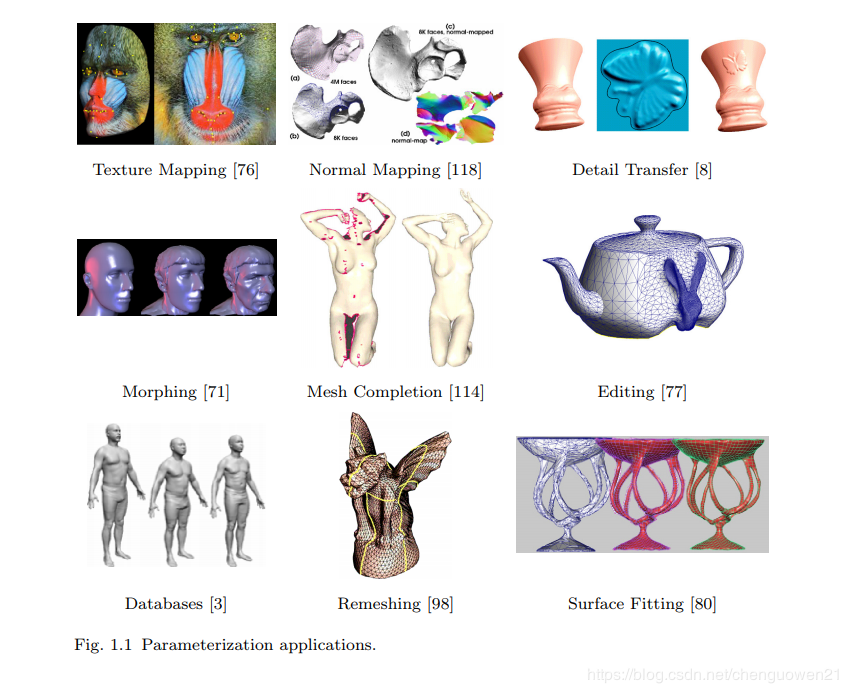
\includegraphics[width=0.8\textwidth]{images/mesh_parameterization_applications.png}
\end{center}

其中存在一些非常重要的概念:
\paragraph{边界}
保持面积或角度的不变,是因为实际需要,如GPU和effect效果的原因,但要完全三角形的映射是完全的,除了类似于折纸(一个平面任意扭曲形成的空间曲面)的网格,
其他网格基本不可能获得完美的保持角度或长度的展开undevelopeable。 

MIPS(Most Isometric Parameterization), 基于扭曲受限的参数化,基于圆模式Circle-Pattern,最小化角度扭曲的参数化

以及最新的LSCM,BFF(Boundary-first-flattening)
